%! Author = zarnold
%! Date = 9/27/20

% Preamble
\documentclass[11pt]{article}
\usepackage[letterpaper]{geometry}
\usepackage{cite}
\usepackage{url}
\usepackage{fancyhdr}
% Packages
\usepackage{amsmath}
\usepackage{graphicx}
\usepackage[english]{babel}
\usepackage{lipsum}
\fancypagestyle{firstpage}
{
\fancyhead[L]{}
\fancyhead[R]{Zach Arnold \linebreak CS 7641 \linebreak Assignment 2}
\setlength{\headheight}{52pt}
}
\graphicspath{./}
\newcommand{\problemone}{One Max Problem}
\newcommand{\problemtwo}{8 Queens Problem}
\newcommand{\problemthree}{Some other problem}
% Document
\begin{document}
    \thispagestyle{firstpage}


    \section{Introduction}
    In this paper I will be exploring the performance and trade-offs of four randomized optimization algorithms: randomized hill climbing,
    simulated annealing, genetic algorithms, and MIMIC against three problems.
    Later in the paper I will reexamine work I did previously in Assigment 1 and attempt to optimize the weights of a multi-layered perceptron using these same
    four algorithms.
    For the purposes of this assignment I used the mlrose library\cite{Hayes19} which was publicly available.
    Note that I made some modifications to the library on my computer to be able to generate timing curves (and I do not
    know how to publish a Python package so I will include instructions for how to get my code in the Readme.)


    \section{Comparison of Randomized Optimization Algorithms}
    This section is dedicated to exploring a comparison of four randomized optimization algorithms against example problems
    which should highlight their relative strenghts and weaknesses.
    The algorithms are randomized hill climbing, simulated annealing, genetic algorithms, and MIMIC.
    I will briefly introduce parameters I will be varying for each algorithm here and then we will compare their performance
    in each problems subsection below.
    \subsubsection*{Randomized Hill Climbing}
    Randomized hill climbing is perhaps one of the more straightforward randomized optimization algorithms to understand.
    It begins in a random location in the search space and looks for random neighbors around that point for an optimal value defined
    by some fitness function.
    If it succeeds in finding such a point the algorithm terminates unless it is configured to restart from a random place elsewhere in the search space.
    The hope is that by randomly restarting we can prevent the algorithm from getting "stuck" in a local maximum and find a global maximum.
    The parameters I am varying are:
    \begin{itemize}
        \item \texttt{max\_attempts} The number of attempts to find a neighbor with better fitness
        \item \texttt{max\_iterations} The number of times to iterations to search (this will usually be lower than \texttt{max\_attempts})
        \item \texttt{restarts} The number of times to randomly restart the above search in a new location in a random location in the search space
    \end{itemize}
    \subsubsection*{Simulated Annealing}
    Simulated Annealing involves a randomized searching technique that involves dynamically constraining and relaxing the values that the algorithm
    will consider to be acceptable as "better fit" by using a schedule to simulate "heating and cooling" or "better or worse fit."
    The theory is that by varying this schedule of heating and cooling that the algorithm will be able to avoid local maxima
    by eventually considering worse values as better outside of the space where the local maximum was in search of a possibly
    better global maximum.
    \begin{itemize}
        \item \texttt{max\_attempts} The number of attempts to find a neighbor with better fitness
        \item \texttt{max\_iterations} The number of times to iterations to search (this will usually be lower than \texttt{max\_attempts})
        \item \texttt{schedule} The decay schedule controls the temperature chance for each iteration of the SA algorithm.
        It can take on three values: Arithmetic, Geometric, and Exponential decay.
        \begin{itemize}
            \item  Arithmetic decay is modeled as $Temp(t) = T_0 - rt$ where $T_0$ is the initial temp and $r$ is some value in (0,1) and represents the rate of arithmetic decay.
            \item Geometric decay is modeled as $Temp(t) = T_0 - r^t$. We expect in this scenario the temperature to decrease much more rapidly.
            \item Exponential decay is modeled as $Temp(t) = T_0 e^{-rt}$ This may look familiar as it is modeled similar to the continuously compounding interest rate formula and should decay the most quickly.
        \end{itemize}
    \end{itemize}
    \subsubsection*{Genetic Algorithm}
    A genetic algorithm takes the concept biological evolution (particularly the concept of "survival of the fittest") and applies it to randomizes search.
    A grouping of randomly selected guesses is selected and the best ones are kept, and the worst fitting elements are replaced by random recombination of the
    elements of of the best performing guesses.
    In this way the algorithm hopes to find a global maximum or "most fit" population by always searching for better and better random recombinations of the the population.
    The parameters I am varying for this algorithm are:
    \begin{itemize}
        \item \texttt{max\_attempts} The number of attempts to find a neighbor with better fitness
        \item \texttt{max\_iterations} The number of times to iterations to search (this will usually be lower than \texttt{max\_attempts})
        \item \texttt{pop\_size} The number of guesses (or population count) to retain at each iteration of the search
        \item \texttt{mutation\_prob} The likelihood of an element in a vector to be randomly recombined if it is in a bad population.
        For example, if this value were 0.1 and the population is a grouping of 10 element vectors, then most likely 1 of the elements will be recombined
        if it is in the "worse performing" group at the end of a "generation" (iteration of the algorithm).
    \end{itemize}
    \subsubsection*{MIMIC}
    MIMIC expands on the concept of Genetic Algorithms combining the best of each generation and replacing the worst in the
    search with the concept of "memory" of previous generations through the use of probability distributions and information theory as
    modeled by Kullback-Libeler divergence.\cite{Isbell97} Thus it should be able to converge much faster to an optimal solution
    than a genetic algorithm for the same problem.
    The parameters I will be varying for this algorithm are:
     \begin{itemize}
        \item \texttt{max\_attempts} The number of attempts to find a neighbor with better fitness
        \item \texttt{max\_iterations} The number of times to iterations to search (this will usually be lower than \texttt{max\_attempts})
        \item \texttt{pop\_size} The number of guesses (or population count) to retain at each iteration of the search
        \item \texttt{keep\_pct} The percentage of guesses to retain between each iteration of the algorithm.
    \end{itemize}
    \subsection{\problemone}
    The \problemone is a fitness function that seeks to maximize a vector $v$ such that:
    \begin{equation}
        \label{oneMax}
        \sum_{i=0}^{n-1} v_i
    \end{equation}
    is a maximum, where $v_i$ is the $i$th component of vector $v$ with length $n$.
    This is a relatively easy optimization problem to understand and it illustrates the effectiveness of MIMIC and Genetic Algorithms
    quite nicely from an efficiency standpoint.
    \linebreak
    \begin{figure}[!htb]
        \begin{minipage}{0.48\textwidth}
            \centering
            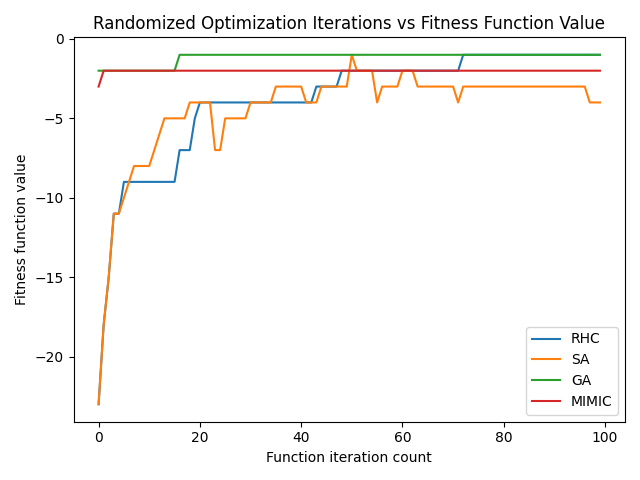
\includegraphics[width=.7\linewidth]{eightqueens.png}
            \caption{Interpolation for Data 1}\label{Fig:Data1}
        \end{minipage}\hfill
        \begin{minipage}{0.48\textwidth}
            \centering
            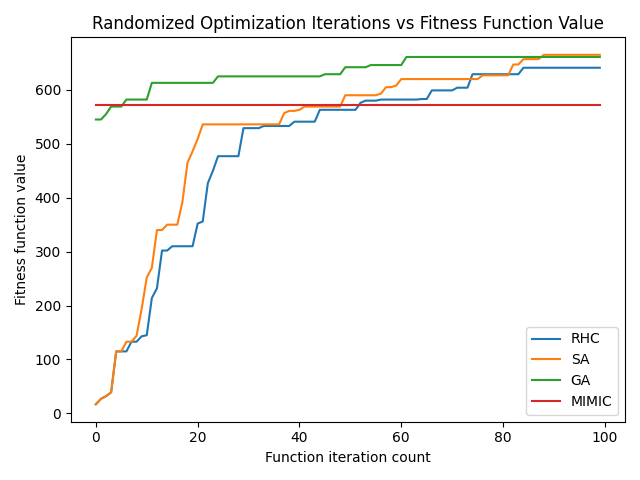
\includegraphics[width=.7\linewidth]{onemax.png}
            \caption{Interpolation for Data 2}\label{Fig:Data2}
        \end{minipage}
    \end{figure}

    \subsection{\problemtwo}
    The eight queens problem is a specific implementation of the n-queens optimization problem.\cite{Russel10} It poses
    an $n x n$ board like in chess where $n$ queens need to be placed such that a minimum number of queens could "attack"
    each other (diagonally, horizontally, or vertically.) So the space to search is a collection of vectors of 8 elements
    where each element is an integer between 0 and 7 and represents where the queen is on that column of the chess board.
    \linebreak

    \subsection{\problemthree}


    \section{Neural Network Weight Optimization}
    \bibliography{assignment2}
    \bibliographystyle{plain}
\end{document}